\documentclass[11pt]{scrartcl}

\usepackage[utf8]{inputenc}
\usepackage[spanish]{babel}

\usepackage{parskip}
\usepackage{graphicx}

\title{Taller de programación III (75.61)\\[0.2em]\Large{Facultad de Ingeniería de la UBA}\\[1em]}
\subtitle{\huge{TP1: Contador de visitas y pruebas de carga\\[0.2em]Informe de pruebas de carga}}
\author{Adrián Barreal\\\small{Segundo cuatrimestre 2021}}
\date{}

\begin{document}
\maketitle
\tableofcontents
\newpage

%========================================================================
%========================================================================
\section{Introducción}

Este documento detalla las pruebas de carga desarrolladas sobre el sitio web institucional cuya estructura fue detallada en el documento de diseño adjunto.
El modelo del usuario para las pruebas de carga y la estructura general de las mismas se detalla en la sección \ref{sec:design}. Se ejecutó una prueba inicial (sección \ref{sec:test-1}) para determinar las capacidades del sistema en su versión original, con los parámetros propuestos en el documento de diseño. En base a los resultados obtenidos se propusieron mejoras para aumentar el rendimiento del sistema, comentadas en la misma sección. Luego se ejecutó una segunda prueba para evaluar la efectividad de las mejoras, obteniendo resultados positivos (sección \ref{sec:test-2}). Algunas conclusiones generales se presentan en la sección \ref{sec:conclusions}.

%========================================================================
%========================================================================
\section{Diseño y ejecución de las pruebas}\label{sec:design}

\begin{figure}
\centering
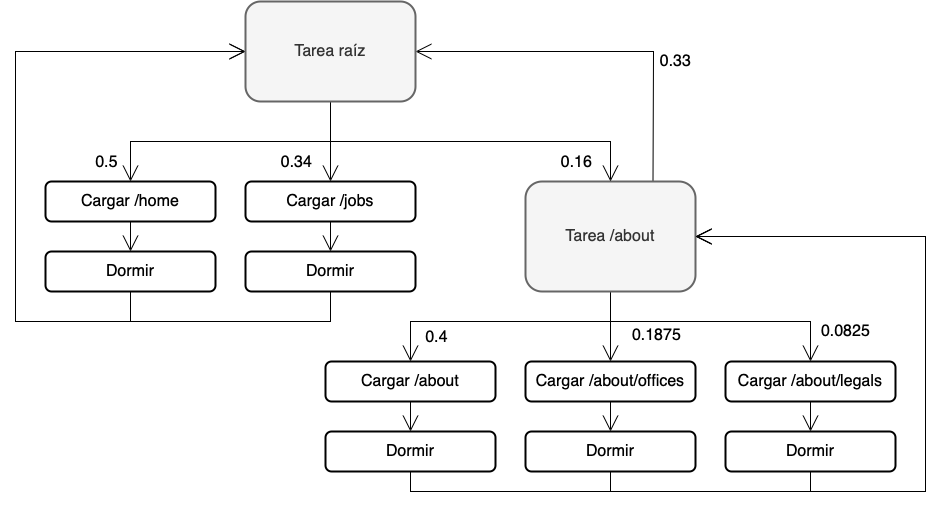
\includegraphics[scale=0.44]{img/user}
\caption{Diagrama de estados que describe el comportamiento del usuario modelo. Los números representan probabilidad de transición.}
\label{fig:user-state}
\end{figure}

Las pruebas de carga fueron desarrolladas usando Locust\footnote{\texttt{https://locust.io}}, un framework para Python diseñado específicamente para la tarea. Cada instancia de prueba simula una cantidad creciente en el tiempo de usuarios concurrentes navegando el sitio web en forma simultánea. El modelo de comportamiento de un usuario se implementó como un script para Locust y se describe como un diagrama de estado en la figura \ref{fig:user-state}. Los usuarios comienzan en el estado inicial ``tarea raíz'' y pueden cambiar de estado siguiendo las aristas del grafo. Los números o pesos que acompañan las aristas representan la probabilidad de transición. Una arista sin peso tiene probabilidad 1 de ejecutarse. Además de las tareas instantáneas ``tarea raíz'' y ``tarea \texttt{/about}'' que son solo conceptuales y no están respaldadas por interacción concreta con la aplicación, hay otros dos tipos de tarea: cargar y dormir, que se describen a continuación:

\begin{itemize}
\item Cargar recurso: Se accede por HTTP al recurso indicado, descargando el contenido HTML. Para emular más adecuadamente el comportamiento del browser, si es la primera vez que el usuario accede a la ruta se procede adicionalmente a extraer y a solicitar todos los recursos estáticos listados en el HTML: imágenes, archivos CSS y archivos JavaScript.
\item Dormir. Se emula el comportamiento de un usuario que pasa una cantidad aleatoria de tiempo en la página a la que accedió, por ejemplo leyendo. Cada página tiene configurados períodos distintos de inactividad (e.g. aquellos pocos usuarios que accedan a la sección de legales podrían pasar una cantidad de tiempo relativamente elevada leyendo el contenido de esa página).
\end{itemize}

Las probabilidades de transición fueron definidas en forma más o menos arbitraria y deberían idealmente surgir de observaciones reales en los datos.

%========================================================================
%========================================================================
\section{Prueba inicial}\label{sec:test-1}

Los principales parámetros que impactan en el rendimiento del sistema, con sus valores iniciales propuestos en el documento de diseño, son los siguientes:
\begin{itemize}
\item Cantidad máxima de instancias del contenedor del sitio web: 2.
\item Cantidad máxima de instancias de la API: 2.
\item Cantidad máxima de instancias del contador de visitas: 2.
\item Cantidad de shards por contador: 100.
\item Todas las instancias fueron provistas de 1 CPU y 1 GB de RAM.
\end{itemize}
Esta primero prueba evalúa el rendimiento del sistema en estas condiciones iniciales.

\subsection{Resultados experimentales}\label{sec:results-1}

El gráfico generado por Locust de la cantidad de usuarios en función del tiempo se presenta en la figura \ref{fig:test-1-users}. El gráfico de la cantidad de pedidos por segundo que generan estos usuarios, así como la cantidad de pedidos que resultan en errores, se muestra en la figura \ref{fig:test-1-requests-per-second}. Se observa que, llegada una cierta cantidad de pedidos por segundo, la aplicación comienza a retornar errores. En la figura \ref{fig:test-1-response-times} puede observarse también un deterioro significativo en el tiempo de respuesta, llegando eventualmente a que al menos el 95\% de los pedidos realizados resultan en timeout.

\begin{figure}
\centering
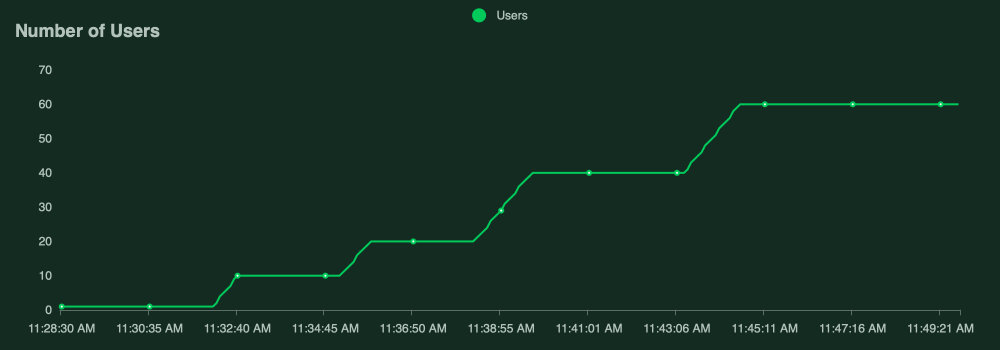
\includegraphics[scale=0.44]{img/usercount}
\caption{Primera prueba: cantidad de usuarios en función del tiempo.}
\label{fig:test-1-users}
\end{figure}

\begin{figure}
\centering
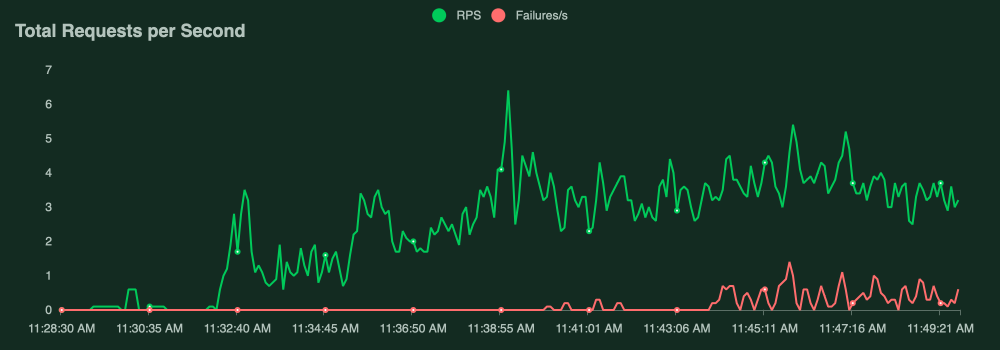
\includegraphics[scale=0.44]{img/requests-per-second}
\caption{Primera prueba: pedidos por segundo y errores por segundo.}
\label{fig:test-1-requests-per-second}
\end{figure}

\begin{figure}
\centering
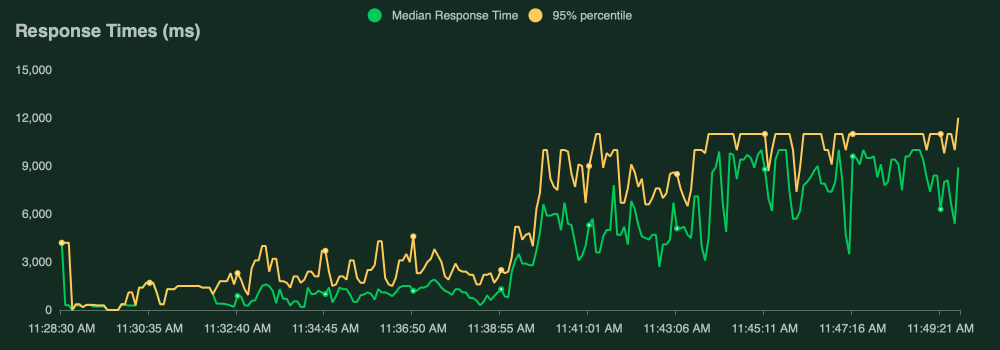
\includegraphics[scale=0.44]{img/response-times}
\caption{Primera prueba: tiempo de respuesta del servidor.}
\label{fig:test-1-response-times}
\end{figure}

El progreso irregular en la figura \ref{fig:test-1-users} se debe a que la intención inicial era duplicar la cantidad de usuarios en cada paso; al observar el rendimiento deteriorado con 40 usuarios, no obstante, se decidió reducir la diferencia hasta la siguiente meseta.

\subsection{Análisis de métricas y resultados}

En los gráficos de las figuras \ref{fig:test-1-users}, \ref{fig:test-1-requests-per-second}, \ref{fig:test-1-response-times} se distinguen vagamente tres regiones: una región de operación normal (con aproximadamente 20 usuarios concurrentes), una región de operación con respuesta notablemente deteriorada pero con una tasa de errores relativamente baja (con aproximadamente 40 usuarios concurrentes) y una región en la que la respuesta del sistema se ve significativamente deteriorada al punto en que hay una cantidad significativa de fallos por segundo por causa de timeout.

Los errores observados se tratan exclusivamente de errores 429. Este es un error que Cloud Run retorna cuando no hay suficientes instancias disponibles para gestionar un pedido dado. Esto quiere decir que en algún punto la aplicación web de cara al usuario no tiene recursos computacionales suficientes para procesar el pedido entrante. En la figura \ref{fig:test-1-cloud-run-cpu} se observa efectivamente que el consumo de CPU de dicho container comienza a subir hasta llegar a 100\% en visible concordancia con el aumento en el tiempo de respuesta. Nótese que la carga en la API permanece relativamente baja a lo largo de todo el experimento.

\begin{figure}[!b]
\centering
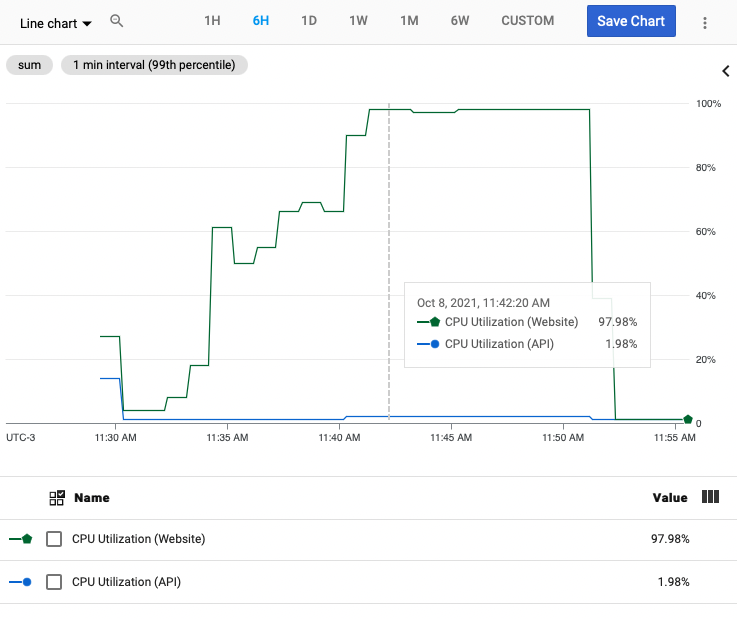
\includegraphics[scale=0.4]{img/cloud-run-cpu}
\caption{Primera prueba: consumpo de CPU en Cloud Run.}
\label{fig:test-1-cloud-run-cpu}
\end{figure}

\begin{figure}
\centering
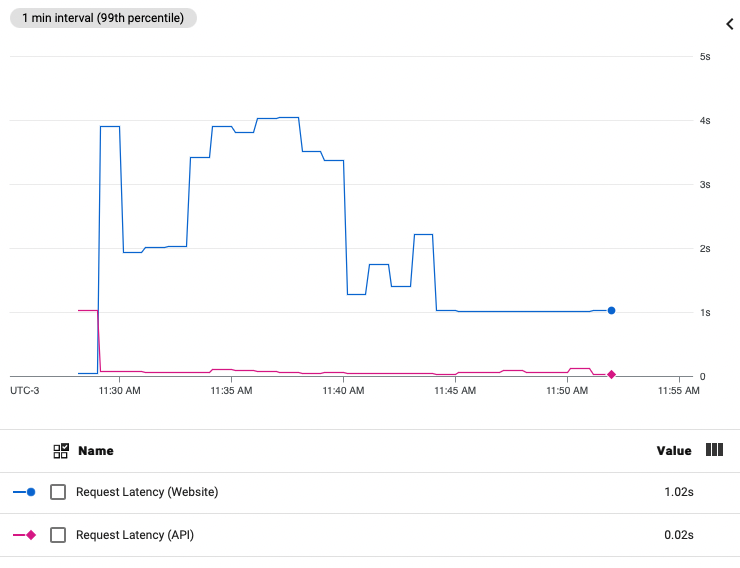
\includegraphics[scale=0.4]{img/cloud-run-request-latency}
\caption{Primera prueba: tiempo de respuesta de Cloud Run.}
\label{fig:test-1-cloud-run-response-time}
\end{figure}

Los gráficos del tiempo de respuesta del contenedor de cara al usuario y de la API se detallan en la figura \ref{fig:test-1-cloud-run-response-time}. Lo importante a observar en este gráfico es lo relativamente poco que tarda la API en responder. Esto indica que el cuello de botella no está en la API.

\textit{\textbf{Nota}: Para el trabajo práctico se incorporó un busy wait al código de algunos controladores del sitio web para simular tareas de carga y procesamiento de datos de varias centenas de milisegundos. Un modelo más adecuado hubiese sido utilizar un sleep bloqueante ya que simularía más adecuadamente el comportamiento de un servidor web que se queda bloqueado esperando la respuesta de, por ejemplo, una base de datos. El busy wait, por otro lado, ocupa la CPU por fracciones importantes de segundo por cada pedido, lo que limita significativamente la cantidad de pedidos por unidad de tiempo que pueden ser atendidos. Dado el busy wait como se implementó, no debería ser posible atender más que unos pocos pedidos por segundo por instancia.}

Se observa por otro lado, en las figuras \ref{fig:test-1-pubsub-subscription} y \ref{fig:test-1-firestore}, que el contador de visitas y Firestore no tienen dificultad  gestionando la cantidad de pedidos entrantes. En la primera se observa que los mensajes entrantes a Pub/Sub son inmediatamente despachados y rápidamente confirmados, sin ningún tipo de acumulación. En la segunda se observa que la cantidad de escrituras por segundo a Firestore no llegan a ser 3; dada la cantidad de shards por contador en uso (100), la probabilidad de colisión en la selección del shard en un segundo dado es diminuta.

\begin{figure}
\centering
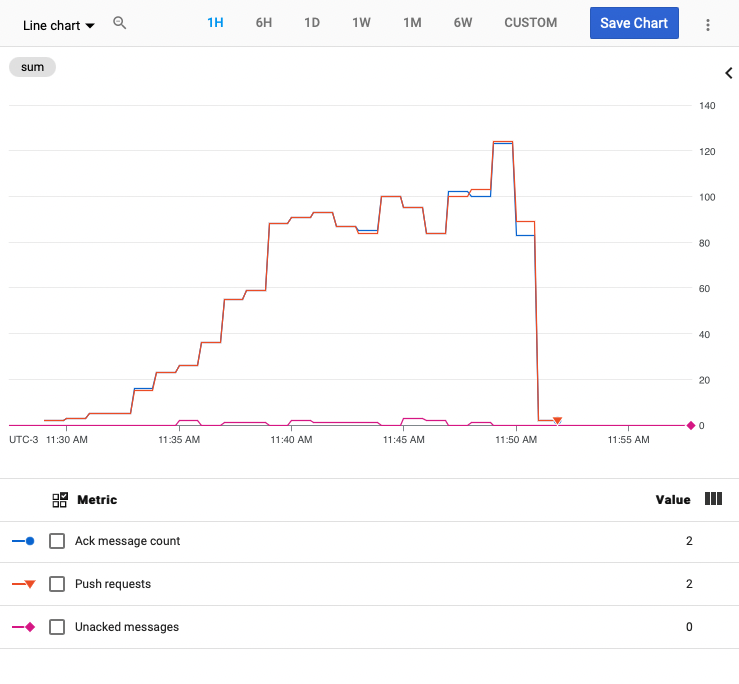
\includegraphics[scale=0.4]{img/pubsub-subscription}
\caption{Primera prueba: mensajes recibidos, despachados y confirmados en Pub/Sub.}
\label{fig:test-1-pubsub-subscription}
\end{figure}

\begin{figure}
\centering
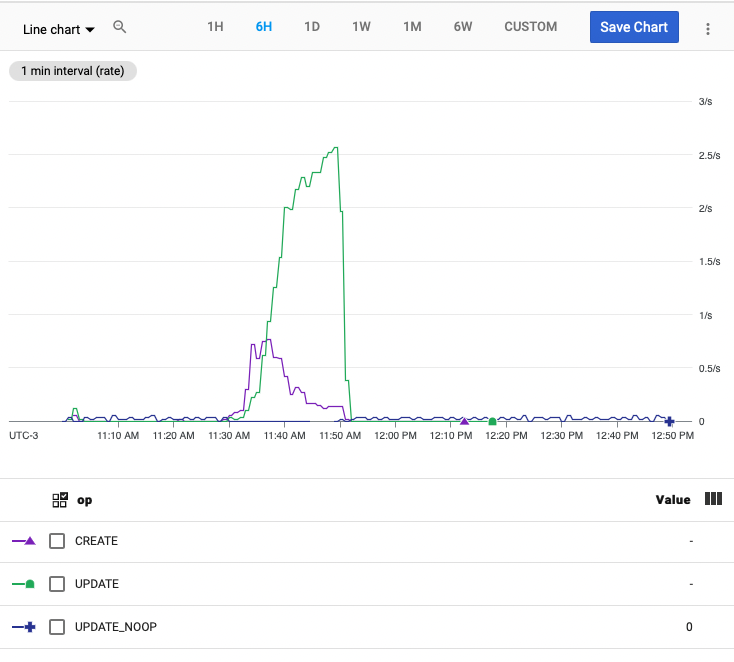
\includegraphics[scale=0.4]{img/firestore}
\caption{Primera prueba: escrituras por segundo a Firestore.}
\label{fig:test-1-firestore}
\end{figure}

\subsection{Mejoras propuestas}\label{sec:improvements}

De las observaciones previas se concluye que para mejorar la capacidad del sistema de tolerar carga es necesario poner foco en mejorar la capacidad del servidor web de cara al usuario. Las mejoras propuestas son las siguientes:

\begin{enumerate}
\item Optimizar el código del contenedor que sirve el contenido web. Esta alternativa no implica costos por mes adicionales de infraestructura.
\item Aumentar la cantidad de instancias del contenedor que sirve el contenido web. Esta opción tendrá un costo económico asociado más allá del costo de desarrollo.
\item Delegar la responsabilidad de servir archivos estáticos a un servicio especializado (e.g. nginx, Google Cloud Storage). Los pedidos por archivos estáticos iniciados por el browser podrían llegar prácticamente en simultáneo, lo cual presentaría un problema observadas las limitaciones de throughput que afectan al servidor web.
\item Disminuir la cantidad máxima de instancias de la API, vista la gran diferencia de consumo de procesador entre los servicios. Se observó en las métricas de Cloud Run que incluso cuando una es suficiente para atender la totalidad de los pedidos en forma eficiente hay una fracción importante del tiempo en la que hay una instancia en estado ``idle''  que fue levantada preventivamente y rápidamente determinada innecesaria por Cloud Run.
\end{enumerate}

No se propone disminuir la cantidad de shards por contador ni de instancias del contador de visitas sin antes evaluar qué impacto tendrán las mejoras propuestas en la carga sobre el sub-sistema de conteo de visitas.

%========================================================================
%========================================================================
\section{Segunda prueba}\label{sec:test-2}

Habiendo implementado las mejoras propuestas en la sección \ref{sec:improvements} se procedió a ejecutar las pruebas de carga nuevamente, obteniendo mejores resultados esta vez. Los parámetros del sistema fueron en esta instancia los siguientes:
\begin{itemize}
\item Cantidad máxima de instancias del contenedor del sitio web: 6 (tres veces más que antes).
\item Cantidad máxima de instancias de la API: 1 (una instancia menos que antes).
\item Cantidad máxima de instancias del contador de visitas: 2 (sin cambios).
\item Cantidad de shards por contador: 100 (sin cambios).
\item Todas las instancias fueron provistas de 1 CPU y 1 GB de RAM (sin cambios).
\item Si bien no se incorporó un proxy reverso para delegar el servicio de archivos estáticos, se simuló la característica eliminando los pedidos del script de Locust.
\end{itemize}

\textit{\textbf{Nota}: Para simular mejoras en el código del contenedor web se redujo el busy wait a la mitad y se agregó en cambio un sleep bloqueante por el total de la cantidad reducida. Si bien el tiempo de respuesta para un pedido individual debería ser el mismo, el hecho de que el sleep sea bloqueante debería tener un impacto positivo en el throughput. En un contexto general esto simularía, por ejemplo, la delegación de cómputo a una base de datos bien provisionada mediante queries más complejos. Esta mejora se evaluó individualmente en una prueba adicional no documentada y se comprobó que el sistema pasa a ser capaz de tolerar 40 usuarios sin deterioro de rendimiento como ocurría inicialmente.}

\subsection{Resultados experimentales}

Gráficos análogos a los presentados en la sección \ref{sec:results-1} se presentan en las figuras \ref{fig:test-2-users}, \ref{fig:test-2-requests-per-second}, \ref{fig:test-2-response-times}. Se observa que la cantidad de pedidos por segundo llega aproximadamente a 12 antes de empezar a observarse errores y tiempos de respuesta deteriorados: entre 3 y 4 veces lo que se obtuvo originalmente.

\begin{figure}
\centering
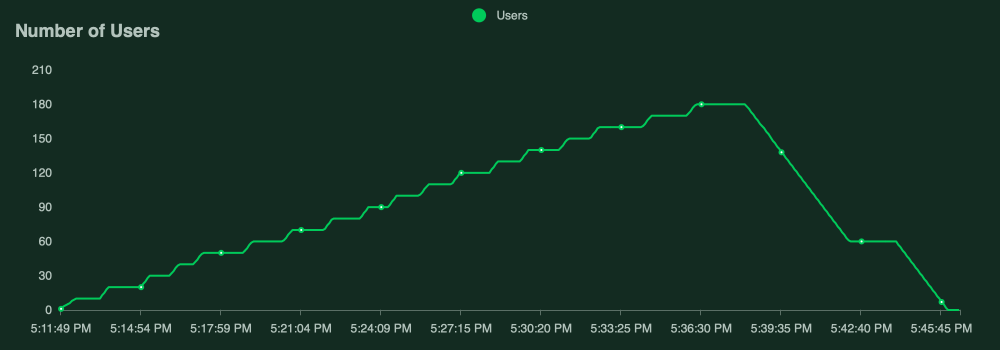
\includegraphics[scale=0.44]{img3/usercount}
\caption{Segunda prueba: cantidad de usuarios en función del tiempo.}
\label{fig:test-2-users}
\end{figure}

\begin{figure}
\centering
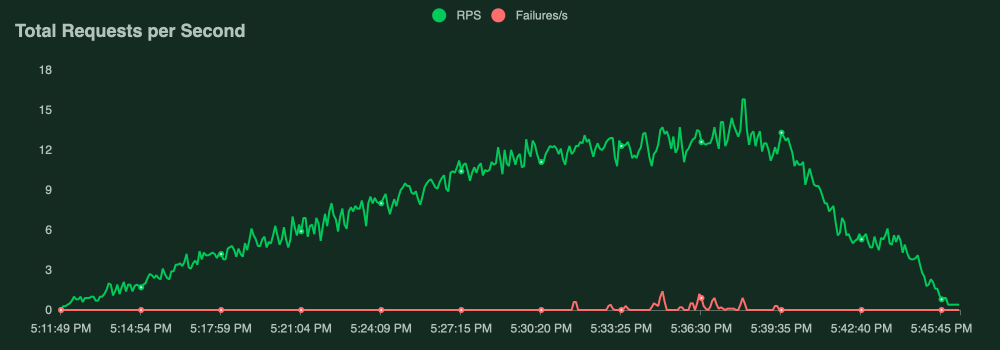
\includegraphics[scale=0.44]{img3/requests-per-second}
\caption{Segunda prueba: pedidos por segundo y errores por segundo.}
\label{fig:test-2-requests-per-second}
\end{figure}

\begin{figure}
\centering
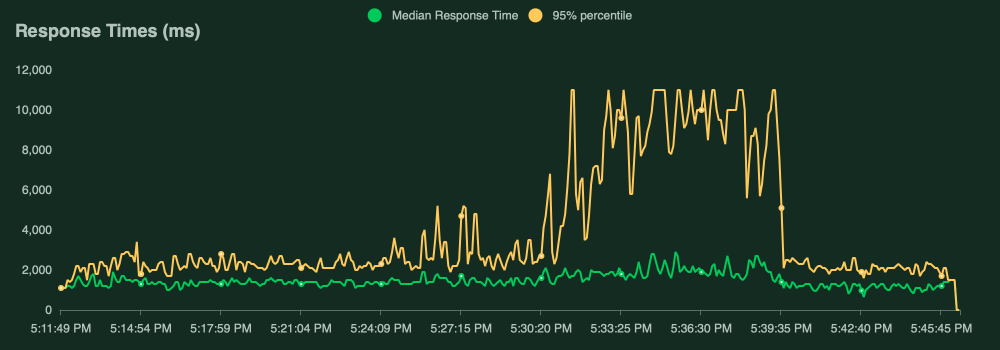
\includegraphics[scale=0.44]{img3/response-times}
\caption{Segunda prueba: tiempo de respuesta del servidor.}
\label{fig:test-2-response-times}
\end{figure}

\subsection{Análisis de métricas y resultados}

Se observa que la mediana del tiempo de respuesta permanece aproximadamente constante en apariencia, lo cual podría indicar que el tiempo de respuesta ante pedidos individuales no se degrada y la limitación sigue estando en el throughput debido a que no hay instancias suficientes para atender la cantidad de pedidos entrantes. Estos pedidos quedan posiblemente acolados en Cloud Run hasta que eventualmente hay instancias libres para procesarlos. Aquellos pedidos que no llegan a ser atendidos antes del tiempo de timeout son descartados por Cloud Run.

\begin{figure}
\centering
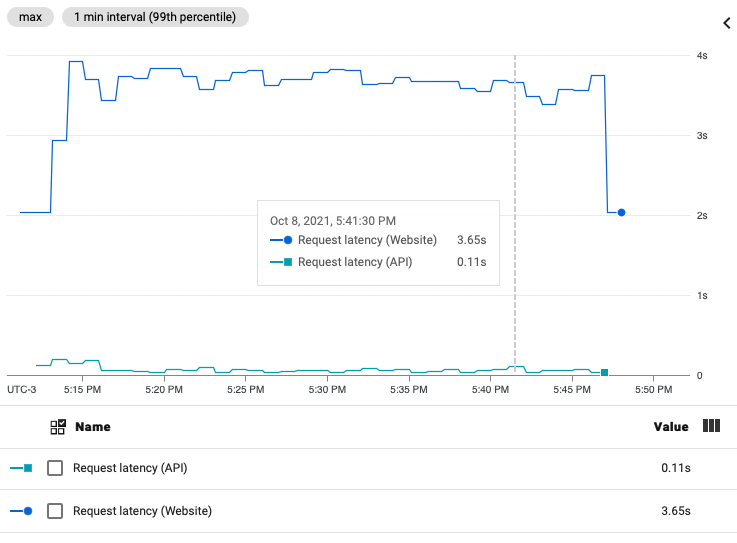
\includegraphics[scale=0.44]{img3/cloud-run-request-latency}
\caption{Segunda prueba: tiempo de respuesta registrado por Cloud Run.}
\label{fig:test-2-cloud-run-response-times}
\end{figure}

Efectivamente, en la figura \ref{fig:test-2-cloud-run-response-times} se observa que según Cloud Run el tiempo máximo de respuesta del servidor web de cara al usuario no llega a superar los 4 segundos en ningún momento durante el experimento. Se sigue observando también que la API responde en forma prácticamente inmediata. Visto que la aplicación no realiza ningún otro pedido a servicio que pudiera convertirse en un cuello de botella (despreciando el tiempo envío de mensajes a Pub/Sub), la limitación actual parecería seguir estando en el tiempo de procesador consumido atendiendo cada pedido individual. Nuevamente, si se deseara seguir mejorando el throughput habría que aumentar la cantidad de instancias en el contenedor del sitio web, u optimizar el algoritmo aún más para hacer uso más eficiente del tiempo de CPU con el que se cuenta.

\begin{figure}
\centering
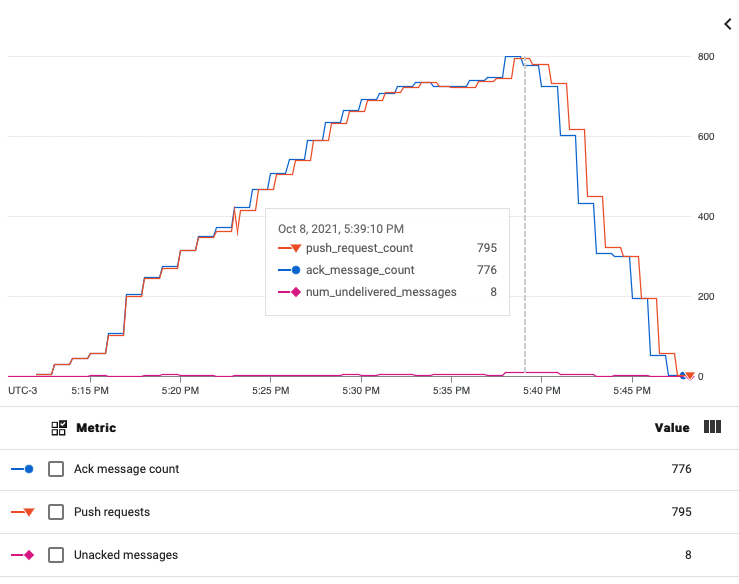
\includegraphics[scale=0.44]{img3/pubsub}
\caption{Segunda prueba: mensajes recibidos, despachados y confirmados en Pub/Sub.}
\label{fig:test-2-pubsub}
\end{figure}

\begin{figure}
\centering
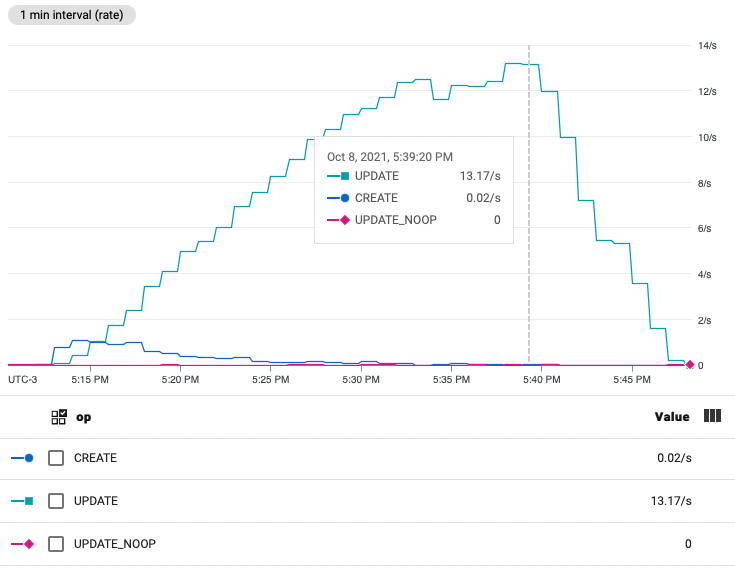
\includegraphics[scale=0.44]{img3/firestore}
\caption{Segunda prueba: escrituras por segundo a Firestore.}
\label{fig:test-2-firestore}
\end{figure}

Resta determinar cómo el aumento en el throughput impacta al sub-sistema de conteo de visitas. La figura \ref{fig:test-2-pubsub} muestra lo que se ve desde el punto de entrada en Pub/Sub. Se observa que el contador tal como está configurado es todavía capaz de atender todos los pedidos entrantes sin acumulación de mensajes. En la figura \ref{fig:test-2-firestore} se observa que la cantidad de escrituras por segundo a Firestore, si bien aumentó, sigue siendo pequeña en relación a la cantidad de shards por contador.

%========================================================================
%========================================================================
\section{Conclusiones}\label{sec:conclusions}

Este experimento permite observar claramente la diferencia entre tiempo de respuesta y throughput. Independientemente del tiempo que se tarde en responder a un pedido individual, si la mayor parte de ese tiempo el proceso permanece bloqueado esperando la respuesta de servicios de back-end la instancia tendrá ciclos de procesador disponibles para atender a una mayor cantidad de clientes en simultáneo. De esto se desprende la importancia de utilizar algoritmos óptimos, de cachear adecuadamente para evitar procesamiento innecesario, de despachar tareas asíncronas a través de colas si es admisible procesar datos en forma diferida, y de evitar repetir tareas de procesamiento si el resultado puede ser compartido, entre otras optimizaciones.

A posteriori se observa que los resultados iniciales podrían haber sido predichos con moderada certeza en forma teórica. Si se conoce el tiempo de procesamiento promedio para cada endpoint, y se conoce el porcentaje de pedidos para cada endpoint, se puede calcular una media ponderada del tiempo de procesamiento por pedido. Razonablemente, si el tiempo promedio de procesamiento por pedido es $T$ milisegundos, se puede estimar la cantidad de pedidos por segundo que puede procesar una instancia con un solo CPU como $1000/T$.

\end{document}